%% This is file `elsarticle-template-1-num.tex',
%%
%% Copyright 2009 Elsevier Ltd
%%
%% This file is part of the 'Elsarticle Bundle'.
%% ---------------------------------------------
%%
%% It may be distributed under the conditions of the LaTeX Project Public
%% License, either version 1.2 of this license or (at your option) any
%% later version.  The latest version of this license is in
%%    http://www.latex-project.org/lppl.txt
%% and version 1.2 or later is part of all distributions of LaTeX
%% version 1999/12/01 or later.
%%
%% Template article for Elsevier's document class `elsarticle'
%% with numbered style bibliographic references
%%
%% $Id: elsarticle-template-1-num.tex 149 2009-10-08 05:01:15Z rishi $
%% $URL: http://lenova.river-valley.com/svn/elsbst/trunk/elsarticle-template-1-num.tex $
%%
%\documentclass[preprint,12pt]{elsarticle}

%% Use the option review to obtain double line spacing
%% \documentclass[preprint,review,12pt]{elsarticle}

%% Use the options 1p,twocolumn; 3p; 3p,twocolumn; 5p; or 5p,twocolumn
%% for a journal layout:
%% \documentclass[final,1p,times]{elsarticle}
%\documentclass[final,1p,times,twocolumn]{elsarticle}
%\documentclass[final,3p,times]{elsarticle}
\documentclass[final,3p,times,twocolumn]{elsarticle}
%% \documentclass[final,5p,times]{elsarticle}
%% \documentclass[final,5p,times,twocolumn]{elsarticle}

%% The graphicx package provides the includegraphics command.
\usepackage{graphicx}
%% The amssymb package provides various useful mathematical symbols
\usepackage{amssymb}
%% The amsthm package provides extended theorem environments
%% \usepackage{amsthm}

%% The lineno packages adds line numbers. Start line numbering with
%% \begin{linenumbers}, end it with \end{linenumbers}. Or switch it on
%% for the whole article with \linenumbers after \end{frontmatter}.
\usepackage{lineno}

%% natbib.sty is loaded by default. However, natbib options can be
%% provided with \biboptions{...} command. Following options are
%% valid:

%%   round  -  round parentheses are used (default)
%%   square -  square brackets are used   [option]
%%   curly  -  curly braces are used      {option}
%%   angle  -  angle brackets are used    <option>
%%   semicolon  -  multiple citations separated by semi-colon
%%   colon  - same as semicolon, an earlier confusion
%%   comma  -  separated by comma
%%   numbers-  selects numerical citations
%%   super  -  numerical citations as superscripts
%%   sort   -  sorts multiple citations according to order in ref. list
%%   sort&compress   -  like sort, but also compresses numerical citations
%%   compress - compresses without sorting
%%
%% \biboptions{comma,round}

% \biboptions{}

\usepackage{import}
\usepackage{amsmath}
\usepackage{multirow}
\usepackage{graphicx,url}
\usepackage{placeins}
\usepackage{adjustbox}
\usepackage[english]{babel}
\usepackage{lipsum}
\usepackage{multicol}
\usepackage{listings}
\usepackage[svgnames]{xcolor} 
\usepackage{caption}
\usepackage{amsmath}
\usepackage{calc} 
\usepackage{array,url,kantlipsum}
\usepackage{lscape}
\usepackage{txfonts}
\usepackage{colortbl}%
  \newcommand{\myrowcolour}{\rowcolor[gray]{0.925}}
\newenvironment{Figure}
  {\par\medskip\noindent\minipage{\linewidth}}
  {\endminipage\par\medskip}
  
\DeclareCaptionFont{white}{\color{white}}
\DeclareCaptionFormat{listing}{\colorbox[RGB]{60,100,180}{\parbox{0.40\textwidth - 2 \fboxsep}{\hspace{8pt}#1#2#3}}}
\captionsetup[lstlisting]{format=listing,labelfont=white,textfont=white, singlelinecheck=false, margin=0pt, font={bf,footnotesize}}

\includeonly{texfiles/planning.tex}

\journal{Systems and Software}

\begin{document}

\begin{frontmatter}

\widowpenalties 1 10000
\raggedbottom

%% Title, authors and addresses

\title{Survey on Workload Techniques for Load, Performance and Stress Tests}
%collaborative approach}

%% use the tnoteref command within \title for footnotes;
%% use the tnotetext command for the associated footnote;
%% use the fnref command within \author or \address for footnotes;
%% use the fntext command for the associated footnote;
%% use the corref command within \author for corresponding author footnotes;
%% use the cortext command for the associated footnote;
%% use the ead command for the email address,
%% and the form \ead[url] for the home page:
%%
%% \title{Title\tnoteref{label1}}
%% \tnotetext[label1]{}
%% \author{Name\corref{cor1}\fnref{label2}}
%% \ead{email address}
%% \ead[url]{home page}
%% \fntext[label2]{}
%% \cortext[cor1]{}
%% \address{Address\fnref{label3}}
%% \fntext[label3]{}


%% use optional labels to link authors explicitly to addresses:
%% \author[label1,label2]{<author name>}
%% \address[label1]{<address>}
%% \address[label2]{<address>}


\author[serpro,unifor,unifor,serpro]{Francisco Nauber Bernardo Gois,Pedro Porf\'irio Muniz de Farias,Andr\'e Lu\'is Vasconcelos Coelho, Thiago Monteiro Barbosa}

\address[serpro]{Serviço Federal de Processamento de Dados,
Avenida Pontes Vieria ,832, Fortaleza, Cear\'a 60130-240}
\address[unifor]{Universidade de Fortaleza, Avenida Pontes Vieria ,832, Fortaleza, Cear\'a 60130-240}

\begin{abstract}
%% Text of abstract
Many software must respond to  thousands or millions of concurrent requests. 
These systems must be properly tested to ensure that they can function correctly under the expected load.  
Load, Performance and Stress Evolutionary testing aims to find test scenarios which produce execution times violating the timing constraints specified. 
The purpose of this paper is propose the use of a approach using  hybrid metaheuristc  in load, performance and stress test models  using Genetic Algorithms, Simulated Annealing and Tabu Search Algorithms. A tool named IAdapter ,  a JMeter Plugin to perform evolutionary load, performance or stress tests, was developed. Two experiments were conducted to validate the proposed approach. The first experiment has been applied in an emulated component and the second experiment has been applied in an installed Moodle application.  In both experiments,  the use of a hybrid metaheurisct  has obtained better fitnesse values.
% * <naubergois@gmail.com> 2015-09-17T00:55:50.180Z:
%
% 
%

% * <naubergois@gmail.com> 2015-09-16T23:54:39.714Z:
%
%  Melhorar frases
%
% ^ <naubergois@gmail.com> 2015-09-16T23:58:15.324Z.
\end{abstract}


\begin{keyword}
Evolutionary Testing \sep Tabu Search \sep Hybrid Metaheuristics
%% keywords here, in the form: keyword \sep keyword

%% MSC codes here, in the form: \MSC code \sep code
%% or \MSC[2008] code \sep code (2000 is the default)

\end{keyword}

\end{frontmatter}

%%
%% Start line numbering here if you want
%%
%\linenumbers
%\section{Introduction}

Many systems must support concurrent
access by hundreds or thousands of users. The failure to scale users results in catastrophic failures and unfavorable media coverage\cite{Jiang2010}. To assure the quality of these systems, performance, stress and load testing is a required testing procedure\cite{Jiang2009}. 

The explosive growth of the Internet has contributed to  increase the need for applications to perform at warp speed. Performance problems have a bad habit of turning up late in the application life cycle, and the later you discover them, the greater the cost to fix them \cite{Molyneaux2009}.
% * <naubergois@gmail.com> 2015-09-16T23:58:29.774Z:
%
%  Alterar frase
%
% ^ <naubergois@gmail.com> 2015-09-16T23:58:46.491Z.
% * <naubergois@gmail.com> 2015-09-16T23:58:52.202Z:
%
% 
%
The use of load testing is an increasingly common practice due to the increasing number of users. In this scenario, the inadequate treatment of a workload generated by concurrent or simultaneously access, generated by system users, can result in highly critical failures and corrosion of the company's image in their customers' view \cite{Draheim2006b} \cite{Jiang2010}. 
% * <naubergois@gmail.com> 2015-09-16T23:58:52.451Z:
%
%  Frase coloquial
%
% ^ <naubergois@gmail.com> 2015-09-16T23:59:03.275Z.

An analysis of sources of failures in the United States Public Switched Telephone Network (PSTN) reported that only 6\% of the outages were overloads. These interruptions have produced  44\% of the PSTN's service's downtime \cite{Kuhn1997}. 

The Load Testing determines the responsiveness, throughput, reliability or scalability of a system under a given workload. The quality of the results of system's load tests is closely linked to the implementation of the workload strategy. The performance of many applications depends on the load applied under different conditions. In some cases, performance degradation and failures arise only in stress conditions \cite{Garousi2010} \cite{Jiang2010}.


Different parts of an application should be tested on various parameters and stress conditions \cite{Babbar2011}. The correct application of a load test should cover most part of application under ordinary conditions (Load or Performance Test) or above the expected load conditions(Stress Test) \cite{Draheim2006b} \cite{Luiz2011} \cite{Fe2004}.

Evolutionary testing is seen as a promising approach for verifying timing constraints \cite{Afzal2009a}. In evolutionary testing the search for the longest execution time is considered a discontinuous, nonlinear optimization problem, with the input domain of the test object as search space, sets of test data as decision variables, and execution times as objective values \cite{Stations}. The main objective of load, performance and stress evolutionary testing is to find test scenarios which produce execution times violating the specified timing constraints \cite{Sullivan}. 

% * <naubergois@gmail.com> 2015-09-17T00:49:26.764Z:
%
%  Rever paragrafo abaixo
%
%
The purpose of this paper is propose the use of a approach using  hybrid metaheuristc   with  Genetic Algorithms, Simulated Annealing and Tabu Search Algorithms  in load, performance and stress evolutionary tests.

The remainder of the paper is organized as follows. Section 2 presents a brief introduction in load, performance and stress tests. Section 3 presents concepts about workload modeling. Section 4 presents a brief introduction about evolutionary test definitions, techniques and state of art. Section 5 presents the IAdapter tool. The Section 6 shows the results of two experiment applied with IAdapter. Conclusions and further work are presented in Section 7.
\section{Planning and Conducting of Research}

In this section, the steps of planning and review of driving are presented in details. The first part of the study was a systematic review. 

A systematic review is a process of assessment of all available research related to a research question or subject of interest. The planning of the systematic review was carried out from the protocol defined by Biolchini \cite{Biolchini2005} \cite{Afzal2009}. Systematic literature review (SLR) is a approach to conducting survey on a research topic. It aims at producing an "engineering" approach with a well-defined methodology so that different investigators can produce survey results effectively and reliably \cite{Kitchenham2007}.


Planning is the starting point for the review, whose main points are the definition of one or more research questions. The activities to conduct the research  includes formulate Research Questions,  The Paper idenfification process (selection of sources to search, search strategies and the use of keywords). 

A  key activity in the planning  of a typical SLR project  is to formulate a set of Research Questions (RQs) before identifying, reading, and analyzing articles of the topic \cite{Jamshidi2013}. 


\subsection{Research Questions}

The work aims to answer two research questions:

First Research Question : How to define a suitable workload for Load Testing to generate realistic loads models (Realistic Workloads)?

Second  Research Question : How to set a suitable workload for Load Testing to fault-inducing loads ?

Third Research Question: In which fora is research on load, performance and stress testing published? 

Fourth Research Question: Which topics for load, performance and stress testing  have been investigated and to what extent?

Fifth Research Question: What types of research are represented and to what extent? 

\subsection{Search strategy}


In this section,we present the search strategy of our paper. 
For each question, keywords were chosen and used in a search strategy. The search strategy for the selection of studies was carried out through search in repositories (ACM, Springer, IEEE, Google Scholar, Science Direct, Mendeley ) , language ( Portuguese and English) and the keywords defined. Using the results, new keywords have been included, feeding back the process. The research strategy included these two practices:

%(Figure \ref{fig:figuraselecao})

\begin{enumerate}
\item Identification of other words and synonyms for terms used in the research questions. This practice is used for minimize the effect of differences in terminologies;
\item The keywords and their possible combinations and synonyms were submitted in the selected repositories search engines; 
\item  Among the results, were excluded studies not related to load, performance and stress tests.
\end{enumerate}

%\begin{figure}[!ht]
%\centering
%\includegraphics[width=0.50\textwidth]{./images/surveybusca2.png}
%\caption{Search Strategy}
%\label{fig:figuraselecao}
%\end{figure}



We used the following search terms:

\begin{itemize}

\item Stress Testing: Search-based Testing, Genetic Algorithms, Stress Testing, Test Tools, Test Automation, Empirical Analysis, Denial of Service, Ramp-Up time, Think Timer,  Response Time, Bandwidth Throttle, Dynamic Stress Testing, Evolutionary, Heuristic, Search-Based, Metaheuristic. optimization, genetic algorithms, genetic programming.
\item Performance Testing: Performance Testing, Web-based Systems, Software Testing, Model-Based Testing, Software Product Line, Regression Testing, Test Failure Prediction, Genetic Metric Selection.
\item Load Testing: Markov chain,  Automatic Test Case Generation Algorithms, Domain-based reliability measure, Fault detection, Load Test suites, load testing, Reliability, Resource allocation mechanisms, Software testing, System degradation.


<<<<<<< HEAD
\end{itemize}


\subsection{Study selection procedure}

The selected studies were filtered by one researcher that used the following inclusion or exclusion criteria:

\begin{itemize}
\item Include: The researcher is sure that the paper is in scope and that it was properly validated using empirical methods.
\item Exclude: The researcher is sure that the paper is out of scope or that the validation was insufficient.
\item Uncertain: The researcher is not sure whether the paper fulfills either the inclusion or exclusion criteria above.
\end{itemize}


\subsection{Classification scheme}

The classification used by the study  is a structure of empirical studies on load,. The scheme consists of six facets, namely quantification approach, abstraction, context, evaluation, research method, and measurement purpose (see Fig. 1). Classification schemes/taxonomies are rated based on a set of quality attributes. A good taxonomy/classification is:
1. Orthogonality: There are clear boundaries between categories, which makes it easy to classify.
2. Defined based on existing literature: The taxonomy/classification is created based on an exhaustive analysis of existing literature in the field.
3. Based on the terminology used in literature: The taxonomy uses terms that are used in existing literature.
4. Complete: No categories are missing, so that existing articles can be classified.
5. Accepted: The community accepts and knows the classification/ taxonomy.


In order to classify each paper selected in accordance with the characteristics of the survey, 



\subsection{Data Extraction and Mapping of Studies}

The relevant articles are sorted into classification scheme, i.e., the actual data extraction takes place. As shown in Figure  the classification scheme evolves while doing the data extraction, like adding new categories or merging and splitting existing categories. 



\section{Load, Performance and Stress Workload: A Brief Introducion}

The term Workload represents  the size of the demand that will be imposed on the application under test in an execution. The metric unit used for define a Workload is dependent on the application domain, such as the length of the video in a transcoding application of multimedia files or the size of the input files to a file compression application \cite{Feitelson2013} \cite{Molyneaux2009} \cite{Goncalves2014}. 

Workload is also defined by the distribution of load between the identified transactions at a given time. Workload helps us study the system behavior identified in several load model. Workload model can be designed for verify predictability, repeatability and scalability of a system \cite{Feitelson2013} \cite{Molyneaux2009}.


Workload modeling is the try to create a simple and general model, which can
then be used to generate synthetic workloads. The goal is typically to be able to create workloads that can
be used in performance evaluation studies. Sometimes, the synthetic workload is supposed to be
similar to those that occur in practice on real systems \cite{Feitelson2013} \cite{Molyneaux2009}.


The workload model is intrinsically linked with the kind of test applied. There are three main tests where these models are usually used: 


\subsection{Performance Testing}

The Performance Test aims at verifying a specified system performance. This kind of test is executed by simulating hundreds or more simultaneous users  over a defined time interval \cite{DiLucca2006}. The purpose of this test is to demonstrate that the system  reaches its performance objectives \cite{Sandler2004}. Other objectives of the performance tests are: Evaluate the adequacy of current capacity	



\subsection{Load Testing}

Load Tests are a kind of test where the system is evaluated in pre-defined load levels \cite{DiLucca2006}. The aim of this test is to reach the performance targets for availability, concurrency, throughput and response time of the system. Load Test is the closest test to real application use \cite{Molyneaux2009}.

\subsection{Stress Testing}

Stress test is a kind of test that verifies the system behaviour against heavy workloads \cite{Sandler2004}. The Stress Testing is executed to evaluate a system beyond its limits. It's used to validate system response in activity peaks and verify if the system is able from recover from these conditions. Stress Tests differs from other kinds of testing  because the system is executed on or beyond its breakpoints. The stress test causes the application or the supporting infrastructure to fail \cite{DiLucca2006} \cite{Molyneaux2009}.



There are two kinds of Workload models: descriptive and generative. The difference is that descriptive models just try to mimic the phenomena observed in the workload, whereas generative models try to emulate the process that generated the workload in the first place \cite{DiLucca2006}. 

\subsection{Descriptive Model}

On descriptive models, one finds different levels of abstraction on one hand, and different levels of faithfulness to the original data on the other hand. The
most strictly faithful models try to mimic the data directly using statistical distribution of data. The most common strategy used in descriptive modeling is to create a statistical
model of an observed workload (Fig. \ref{fig:descriptivemodel}). This model is applied to all the workload
attributes, e.g. computation, memory usage, I/O behavior, communication, etc \cite{DiLucca2006}. The Fig. \ref{fig:descriptivemodel} shows a simplified workflow of a descriptive model. The workflow has six phases. In first phase, the user uses the system in the production environment. In second phase, the tester collects user's data, like logs, clicks and preferences, in the system . The third phase consists in developing a model to emulate the user's behaviour. The fourth phase is made up of the execution of the test, emulation of the user's behaviour and log's gathering.

\begin{figure}[!ht]
\centering
\includegraphics[width=0.5\textwidth]{./images/workloadmodel1.png}
\caption{Workload modeling based on statistical data \cite{DiLucca2006}}
\label{fig:descriptivemodel}
\end{figure}

\subsection{Generative Model}

Generative models are indirect, in the sense that they do not model the statistical distributions. Instead, they describes how users will behave and when they generate the workload. An important benefit of the generative approach is
that it facilitates manipulations of the workload. It is often desirable to be able to change the workload conditions as part of the evaluation. Descriptive models do not offer any option regarding how to do so. But with generative models, we can modify the workload-generation process to fit the desired conditions \cite{DiLucca2006}. The difference between the workflows of descriptive and generative models is that user behavior is not collected from logs, but simulated from a model that can receive feedback from the test execution (Fig. \ref{fig:generativemodel}).

\begin{figure}[!ht]
\centering
\includegraphics[width=0.5\textwidth]{./images/workloadmodel2.png}
\caption{Workload modeling based on Generative Model \cite{DiLucca2006}}
\label{fig:generativemodel}
\end{figure}
\input{texfiles/mapresults.tex}
\section{Load, Performance and Stress Cloud Testing}


Cloud computing alters the way of obtaining computing resources, managing and delivering software, technologies and solutions. Meanwhile, cloud computing also brings new issues, challenges, and needs in cloud-based application testing and evaluation. In the past decades, there were numerous published technical papers focusing on scalability analysis and performance evaluation. 

The presented research work found one systematic review on cloud software testing:


\begin{itemize}
\item 5W+1H pattern: A perspective of systematic mapping studies and a case study on cloud software testing \cite{Jia2015}.
\end{itemize}

The Figure \ref{fig:surveycloud}  shows a comparison between the  researches found in the presented research work. The x axis represents the kind of cloud used ( SaaS, PaaS  or IaaS )  and the y axis presents the type of workload strategy used by each research (Generativive or Descriptive Workload). The Figure also divides the researches by the type technique used in each paper.


\begin{figure}[!ht]
\centering
\includegraphics[width=0.5\textwidth]{./images/SurveyFiguraCloud3.png}
\caption{Distribution of the researches over kind of cloud}
\label{fig:surveycloud}
\end{figure}



\subsection{Papers found in the presented research work}

This subsection presents details about the papers found in the presented research work.

Gao et. al. proposes  a new formal graphic models and metrics to test SaaS performance and analyze system scalability in clouds. This paper presents a analytic models in a radar chart graphic format to evaluation for system performance and scalability of SaaS applications in a cloud.  The paper consider three types of system loads\cite{Gao2011}.

\begin{itemize}
\item The communication traffic load:  The amount of incoming and outgoing communication messages and transactions in a given time unit during system performance and evaluation.
\item The system user access load during:The number of concurrent users who access the system in a given time unit.
\item The system data load: the underlying
system data store access load, such as the number of data
store access, and data storage sizing.
\end{itemize}


Snellman et. al. propose the ASTORIA framework to identify problems using Record and Playback User Actions. The ASTORIA is a framework for automatic performance and scalability testing of Rich Internet Applications.\cite{Snellman2011}.

Tsai et. al. propose scalability metrics that can be used to test the scalability of SaaS applications.

Jayasinghe presents Expertus, a tool to automate large scale distributed experiment studies in IaaS clouds. The Expertus have the goal of addressing three challenges discussed in Section II.
\section{Evolutionary Test in Load, Performance and Stress Tests}

The search for the longest execution time is regarded as a discontinuous, nonlinear, optimization problem, with the input domain of the system under test as search space \cite{Sullivan}. The main objective of evolutionary testing in performance,stress and load tests is to find test scenarios which produce execution times violating the timing constraints specified. If a temporal error is found, the test was successful \cite{Sullivan}. The application of evolutionary algorithms to load, performance and stress tests involves finding the best and worst case execution times (BCET, WCET) to determine if timing constraints are fulfilled \cite{Afzal2009a}. 

Evolutionary tests uses a cost (fitnesse) function to select the best individuals. There has two measurement units normally associated with the fitnesse function in load, performance or stress test: Processor Cycles and Execution Time. The Processor Cycles approach describes a fitness function in terms of processor cycles. The Execution Time approach involves executing the application under test measuring the execution time \cite{Afzal2009} \cite{tracey2000search}.
% * <naubergois@gmail.com> 2015-09-17T01:17:52.488Z:
%
%  Rever esse paragrafo
%
The Figure \ref{fig:comparison}  shows a comparison between the presented research work and the load, performance and stress test researches presented by Afzal et. al. \cite{Afzal2009}. Afzal's work was added with some of the latest research in the area (\cite{Garousi2006} \cite{Garousi2010}). The x axis represents the type of tool used ( Prototype or Functional Tool )  and the y axis presents the metaheuristic used by each research (Genetic Algorithm, Tabu Search, Simulated Annnealing or a Customized Algorithm). The Figure also divides the researches by the type of function fitnesse (Execution Time or Processor Cycles). Most research is limited to making prototypes on genetic algorithms. The presented research work is distinguished from others by having a functional tool using a hybrid approach. 

% * <naubergois@gmail.com> 2015-09-17T01:22:09.554Z:
%
%  Customized Algorithm
%

\begin{figure}[h]
\centering
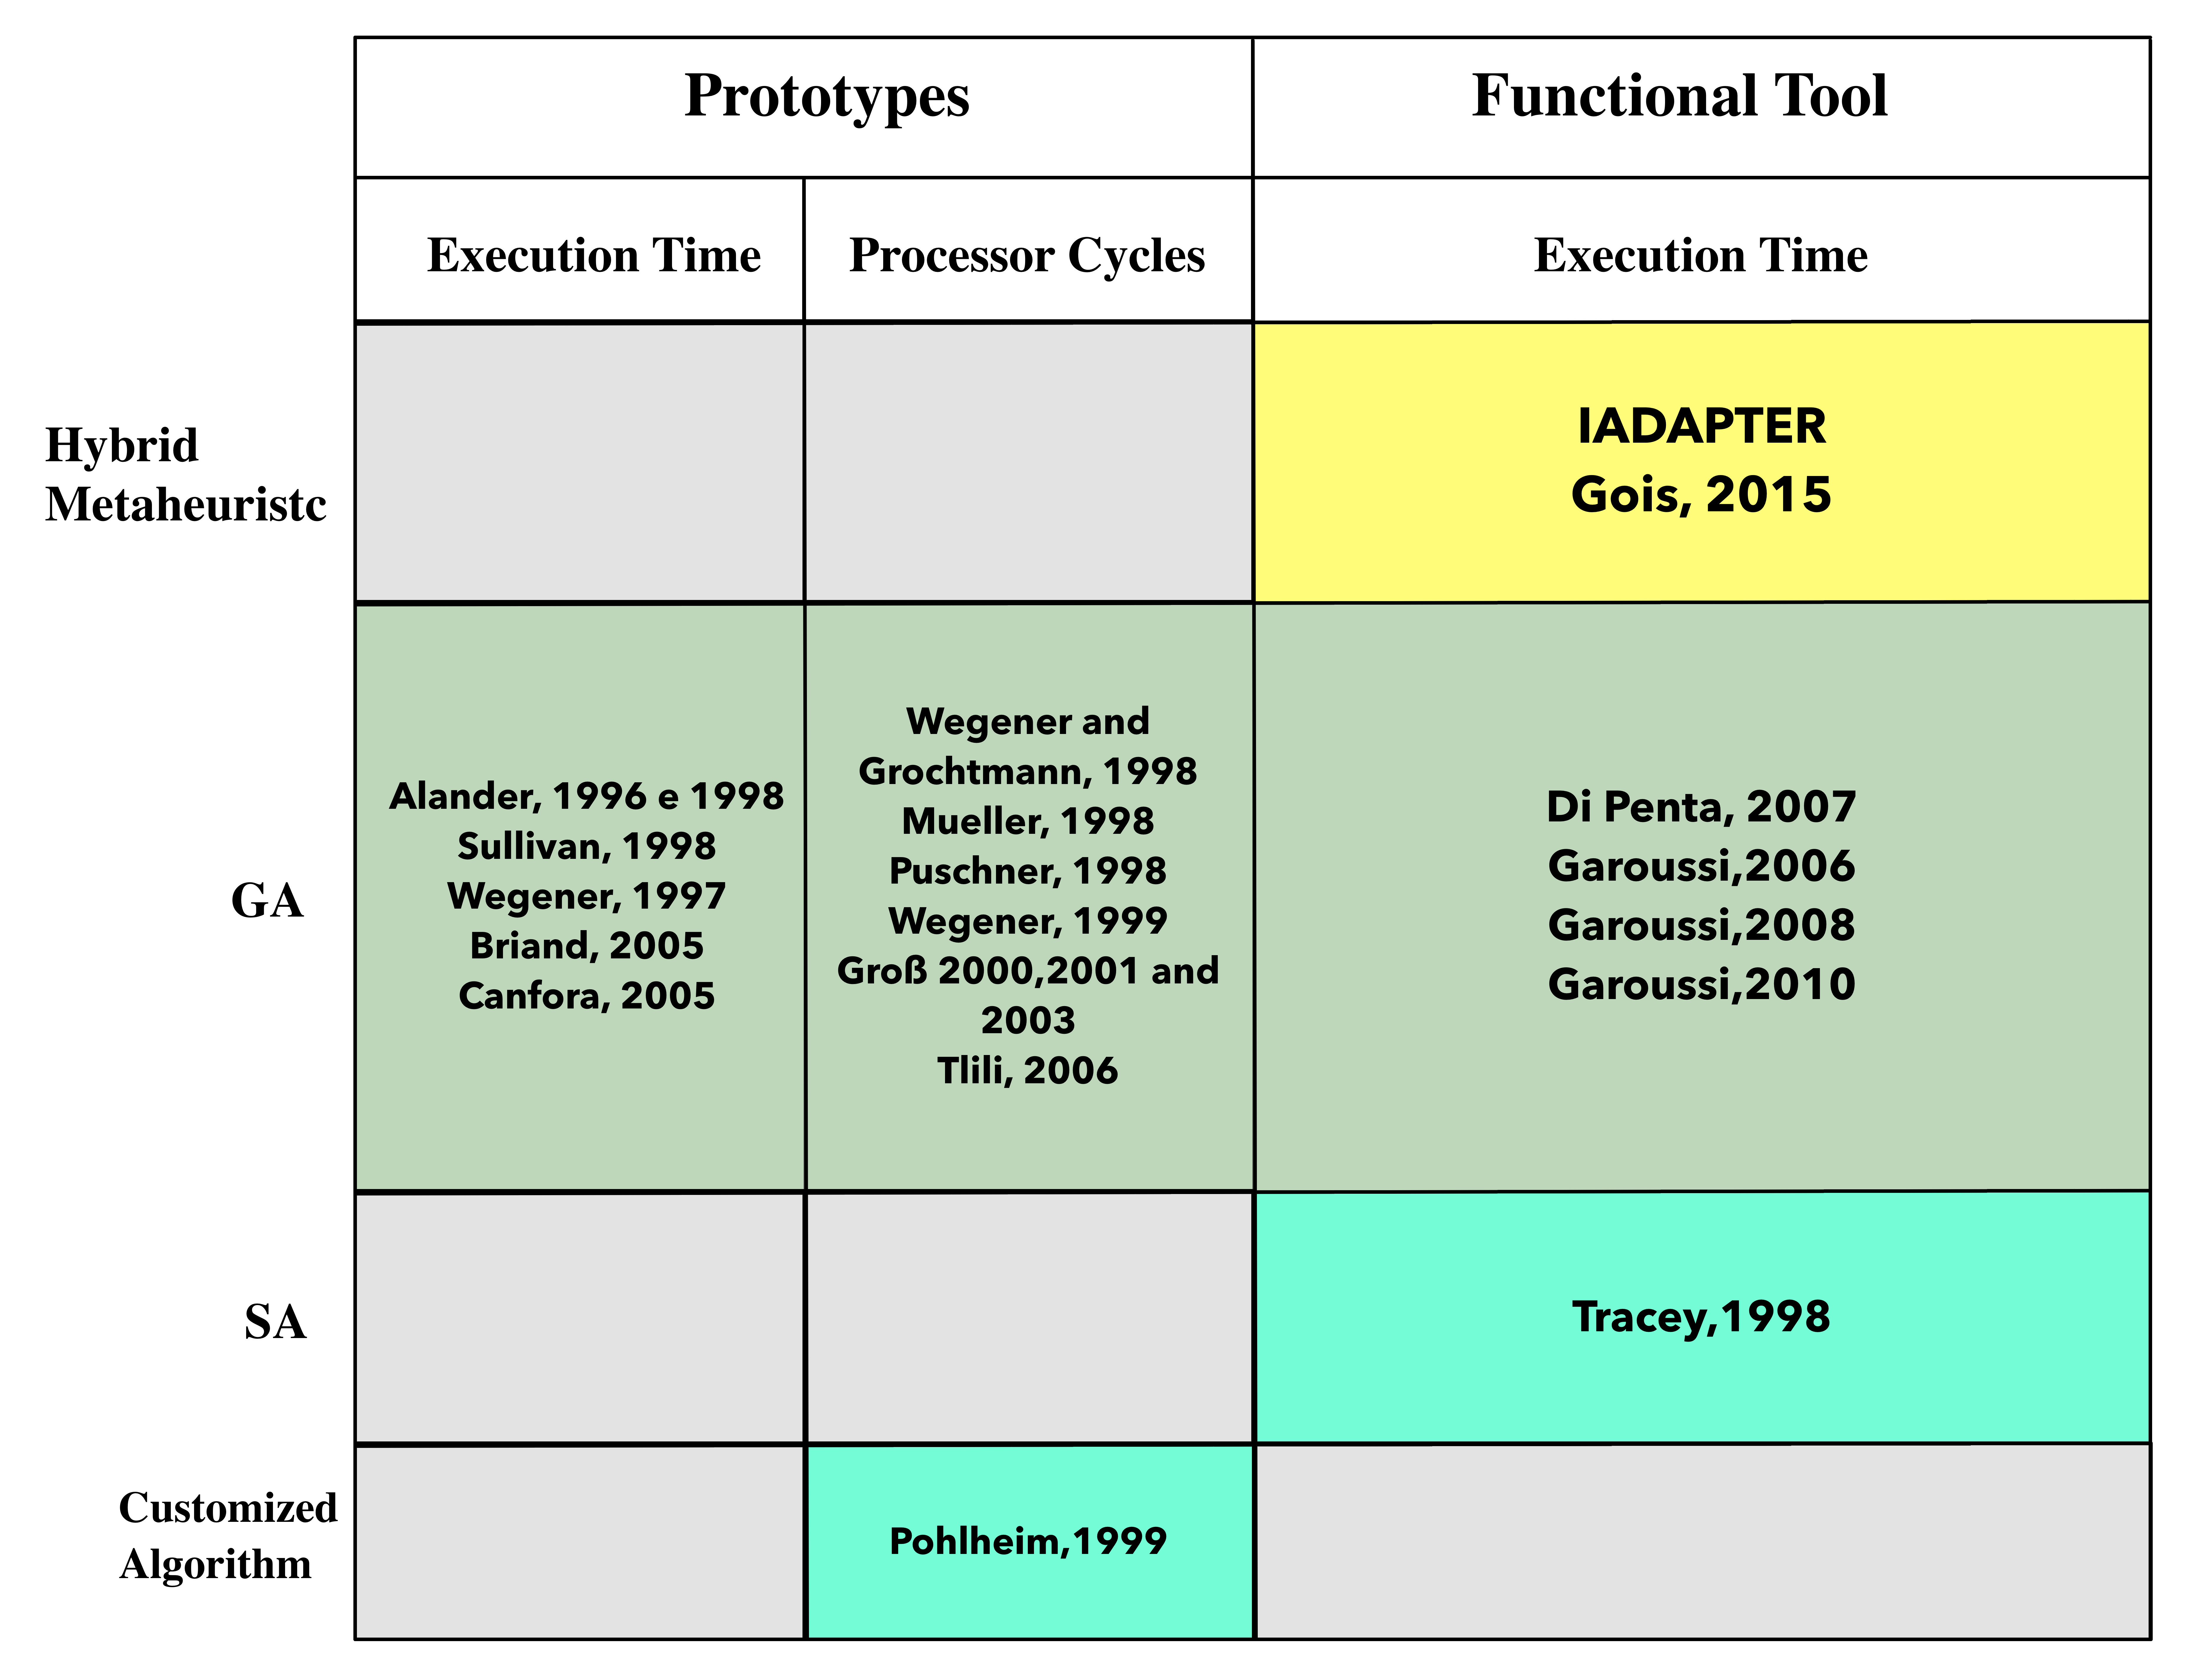
\includegraphics[width=0.5\textwidth]{./images/comparativo1.png}
\caption{
Distribution of the researches over range of applied metaheuristics}
\label{fig:comparison}
\end{figure}
\section{WorkLoad Analysis}
%\section{IAdapter}

IAdapter is a JMeter Plugin to perform evolutionary load, performance or stress tests. JMeter is a desktop application, designed to test and measure the performance and functional behavior of applications \cite{Nevedrov2007}.

The IAdapter plugin makes it possible to create a generative model that evolves during the test. The IAdapter model uses metaheuristic algorithms with three goals:

\begin{itemize}
\item find test scenarios with service level service limits;
\item find test scenarios that show performance errors;
\item automate the performance test execution;
\end{itemize}

In this section, We presents details about the use of Metaheuristcs algorithms( objective (fitnesse) , initial population and genotype representation) and IAdapter Components.

\subsection{Use of MetaHeuristics Algorithms}

The plugin uses Genetic Algorithms, Simulated Annealing and TABU Search algorithms in two different approaches. The first approach uses the three algorithms independently. The second approach uses the three algorithms collaboratively (Hybrid Metaheuristic approach).

In the first approach , the algorithms do not share their best individuals among themselves. Each algorithm evolves in a separate way (Fig. \ref{fig:firstaproach}). The second approach use the algorithms in a collaborative mode (Hybrid Metaheuristic). In this approach, the three algorithms share their best individuals found (Fig. \ref{fig:secondapproach} ).

\begin{figure}[h]
\caption{Use of the algorithms independently}
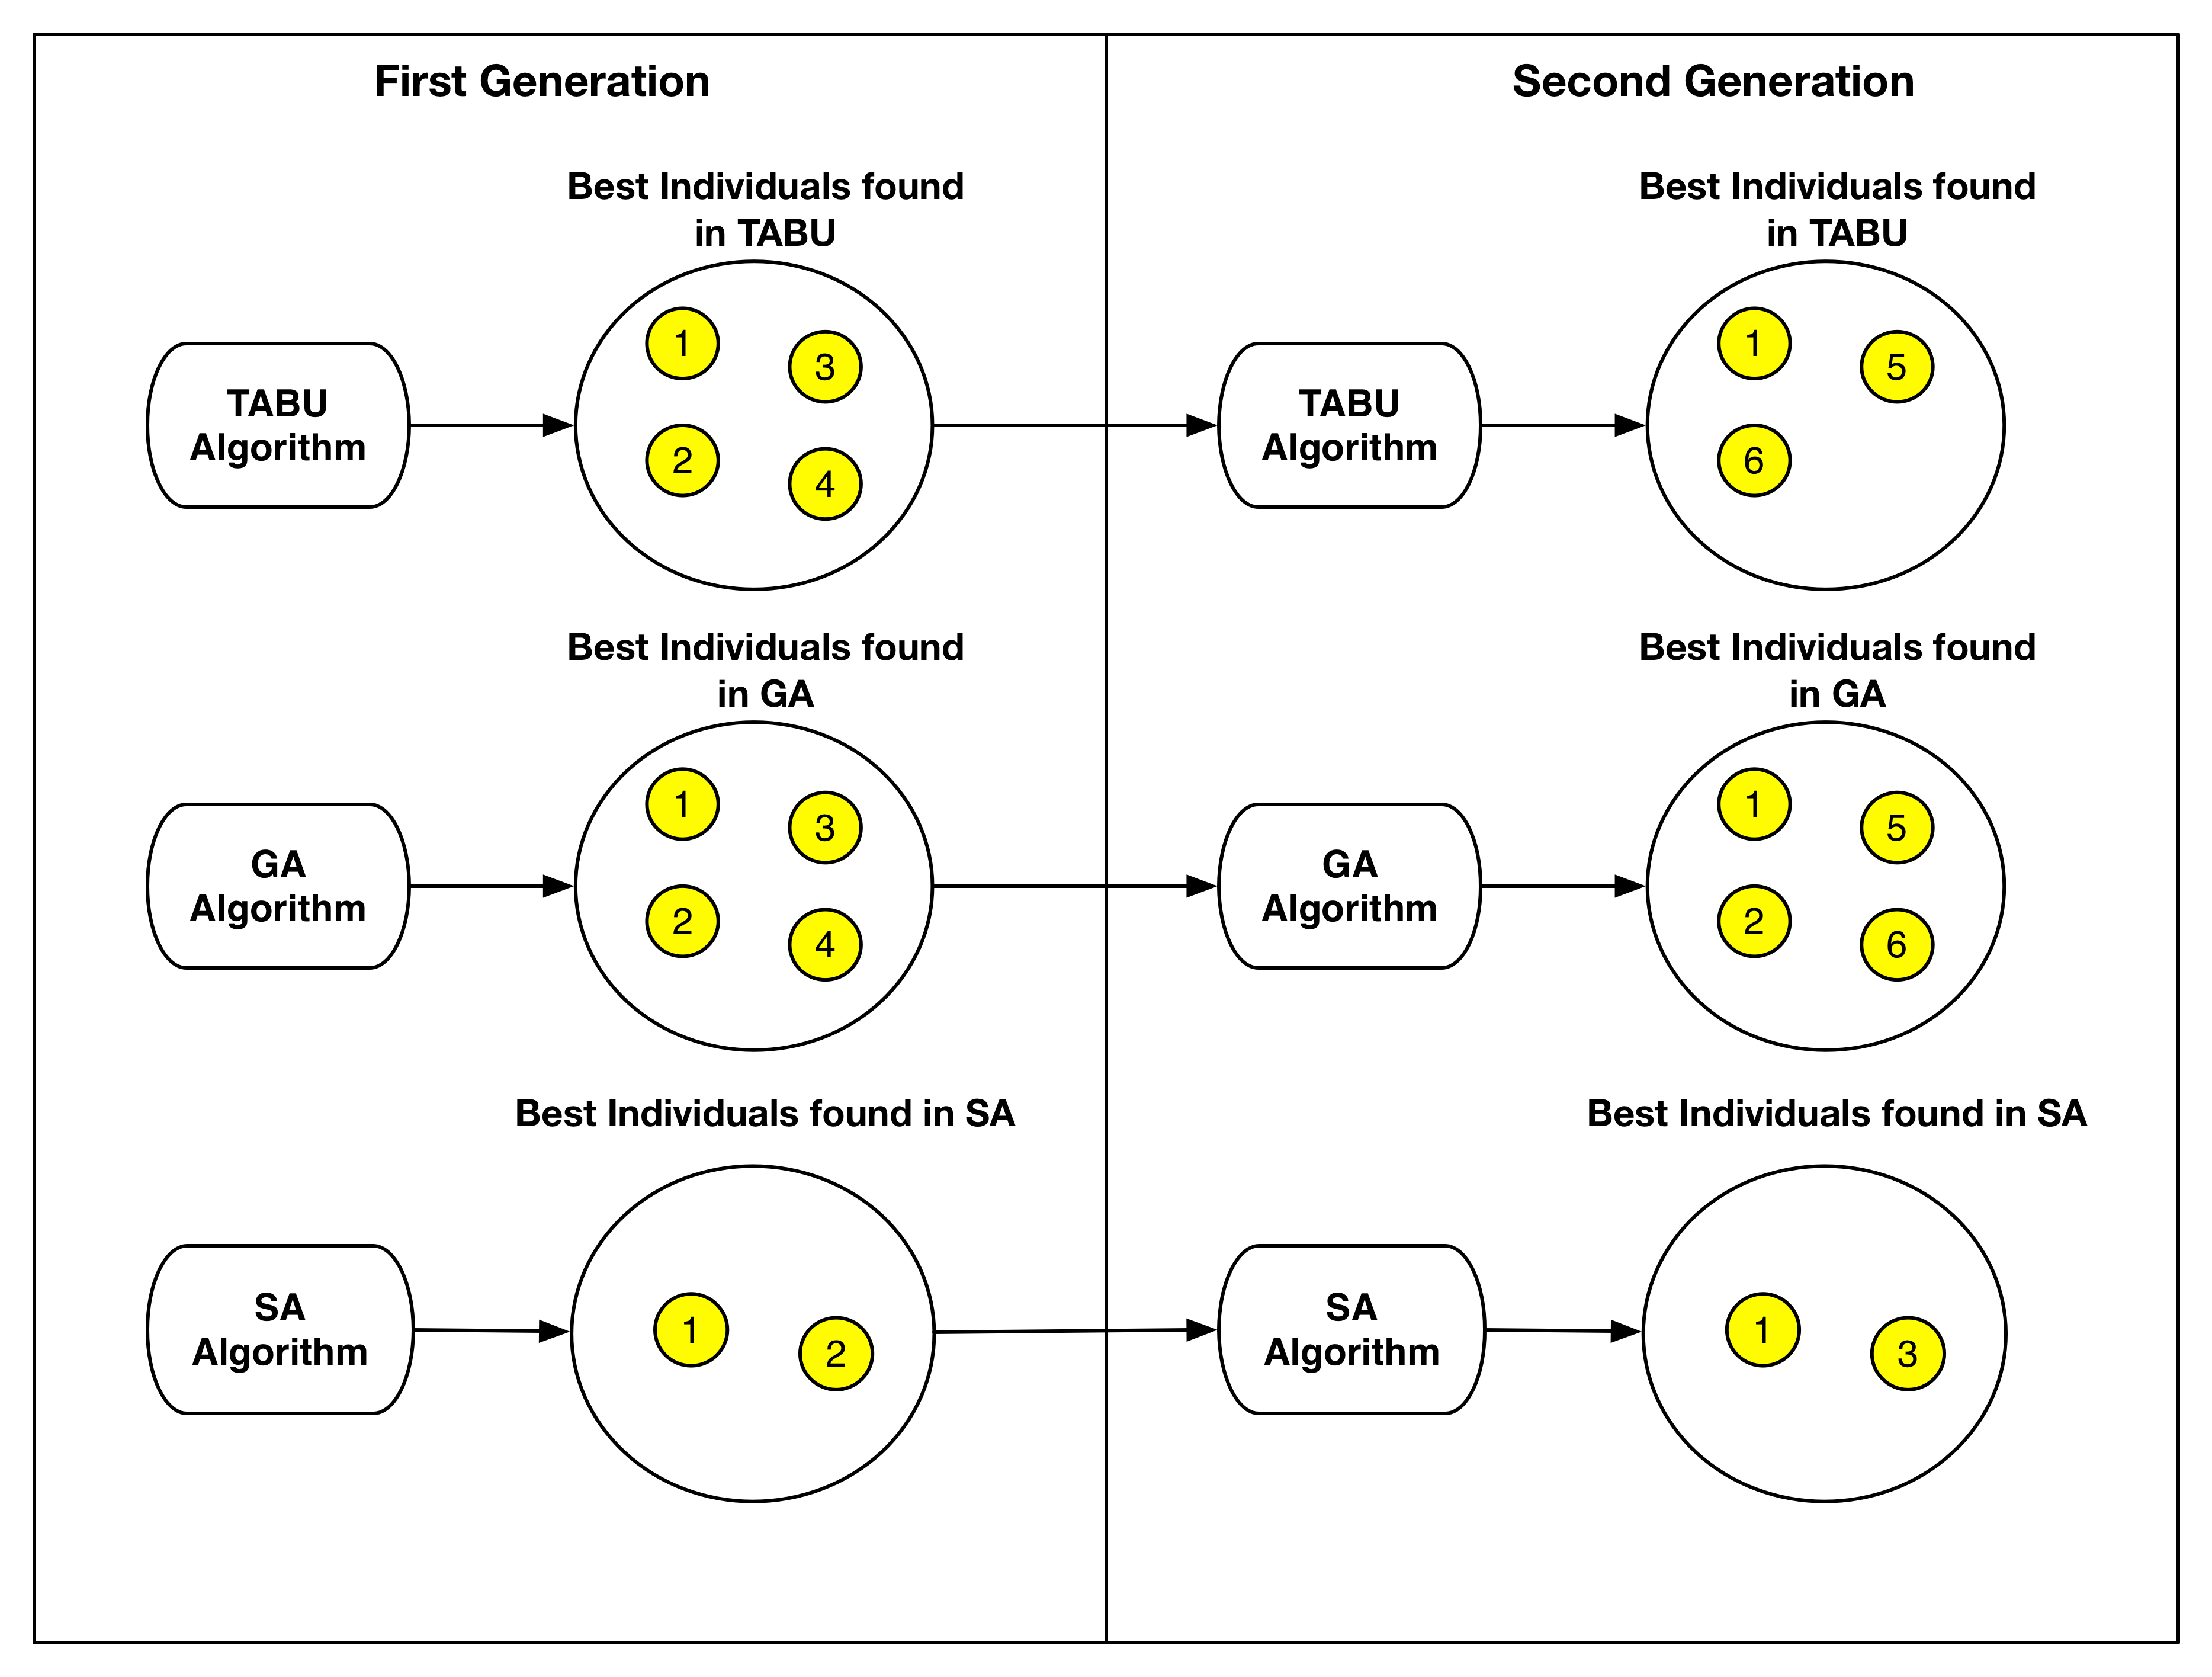
\includegraphics[width=0.5\textwidth]{./images/independ.png}
\label{fig:firstaproach}
\end{figure}
\begin{figure}
\caption{Second approach of use combinatorial optimization algorithms}
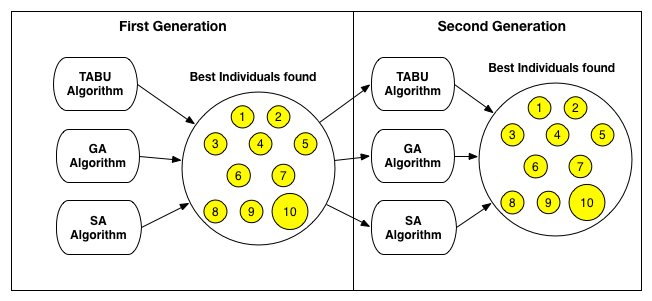
\includegraphics[width=0.5\textwidth]{./images/collaborative.png}
\label{fig:secondapproach}
\end{figure}

\subsubsection{Initial population}

The strategy use by the plugin to instantiate the initial population is to generate 50\% of the individuals randomically and 50\% of the initial population are distributed in three  ranges of values:

\begin{itemize}
\item 30\% of the maximum allowed users in the test ;
\item 60\% of the maximum allowed users in the test; and
\item 90\% of the maximum allowed users in the test.
\end{itemize}


\subsubsection{Genotype representation}

The Genotype representation is composed by a linear vector with 23 genes. The first gene represents the name of individual. The second gene presents the  algorithm (Genetic Algorithm, Simulated Annealing or Tabu Search) used by the individual. The third gene represents the type of test (Load, Stress or Performance). Next genes represent 10 scenarios and their numbers of users. Each scenario is an atomic operation, the scenario must log in the application, run the task goal and undo any changes performed, returning the application to it's original state. 

The Fig. \ref{fig:genomarepresentation} presents the genome representation and  a example using the crossover operation. In the example, the genotype 1 has the Login scenario with 2 users; the Form scenario with 0 users and the Search scenario with 3 users. The genotype 2 has the Delete scenario with 10 users; the Search scenario with 0 users and the Include scenario with 5 users. After the crossover operation, We obtain a genotype with  Login scenario with 2 users; the Search scenario with 0 users and the Include scenario with 5 users.

\begin{figure}[h]
\caption{Genotype representation and crossover example}
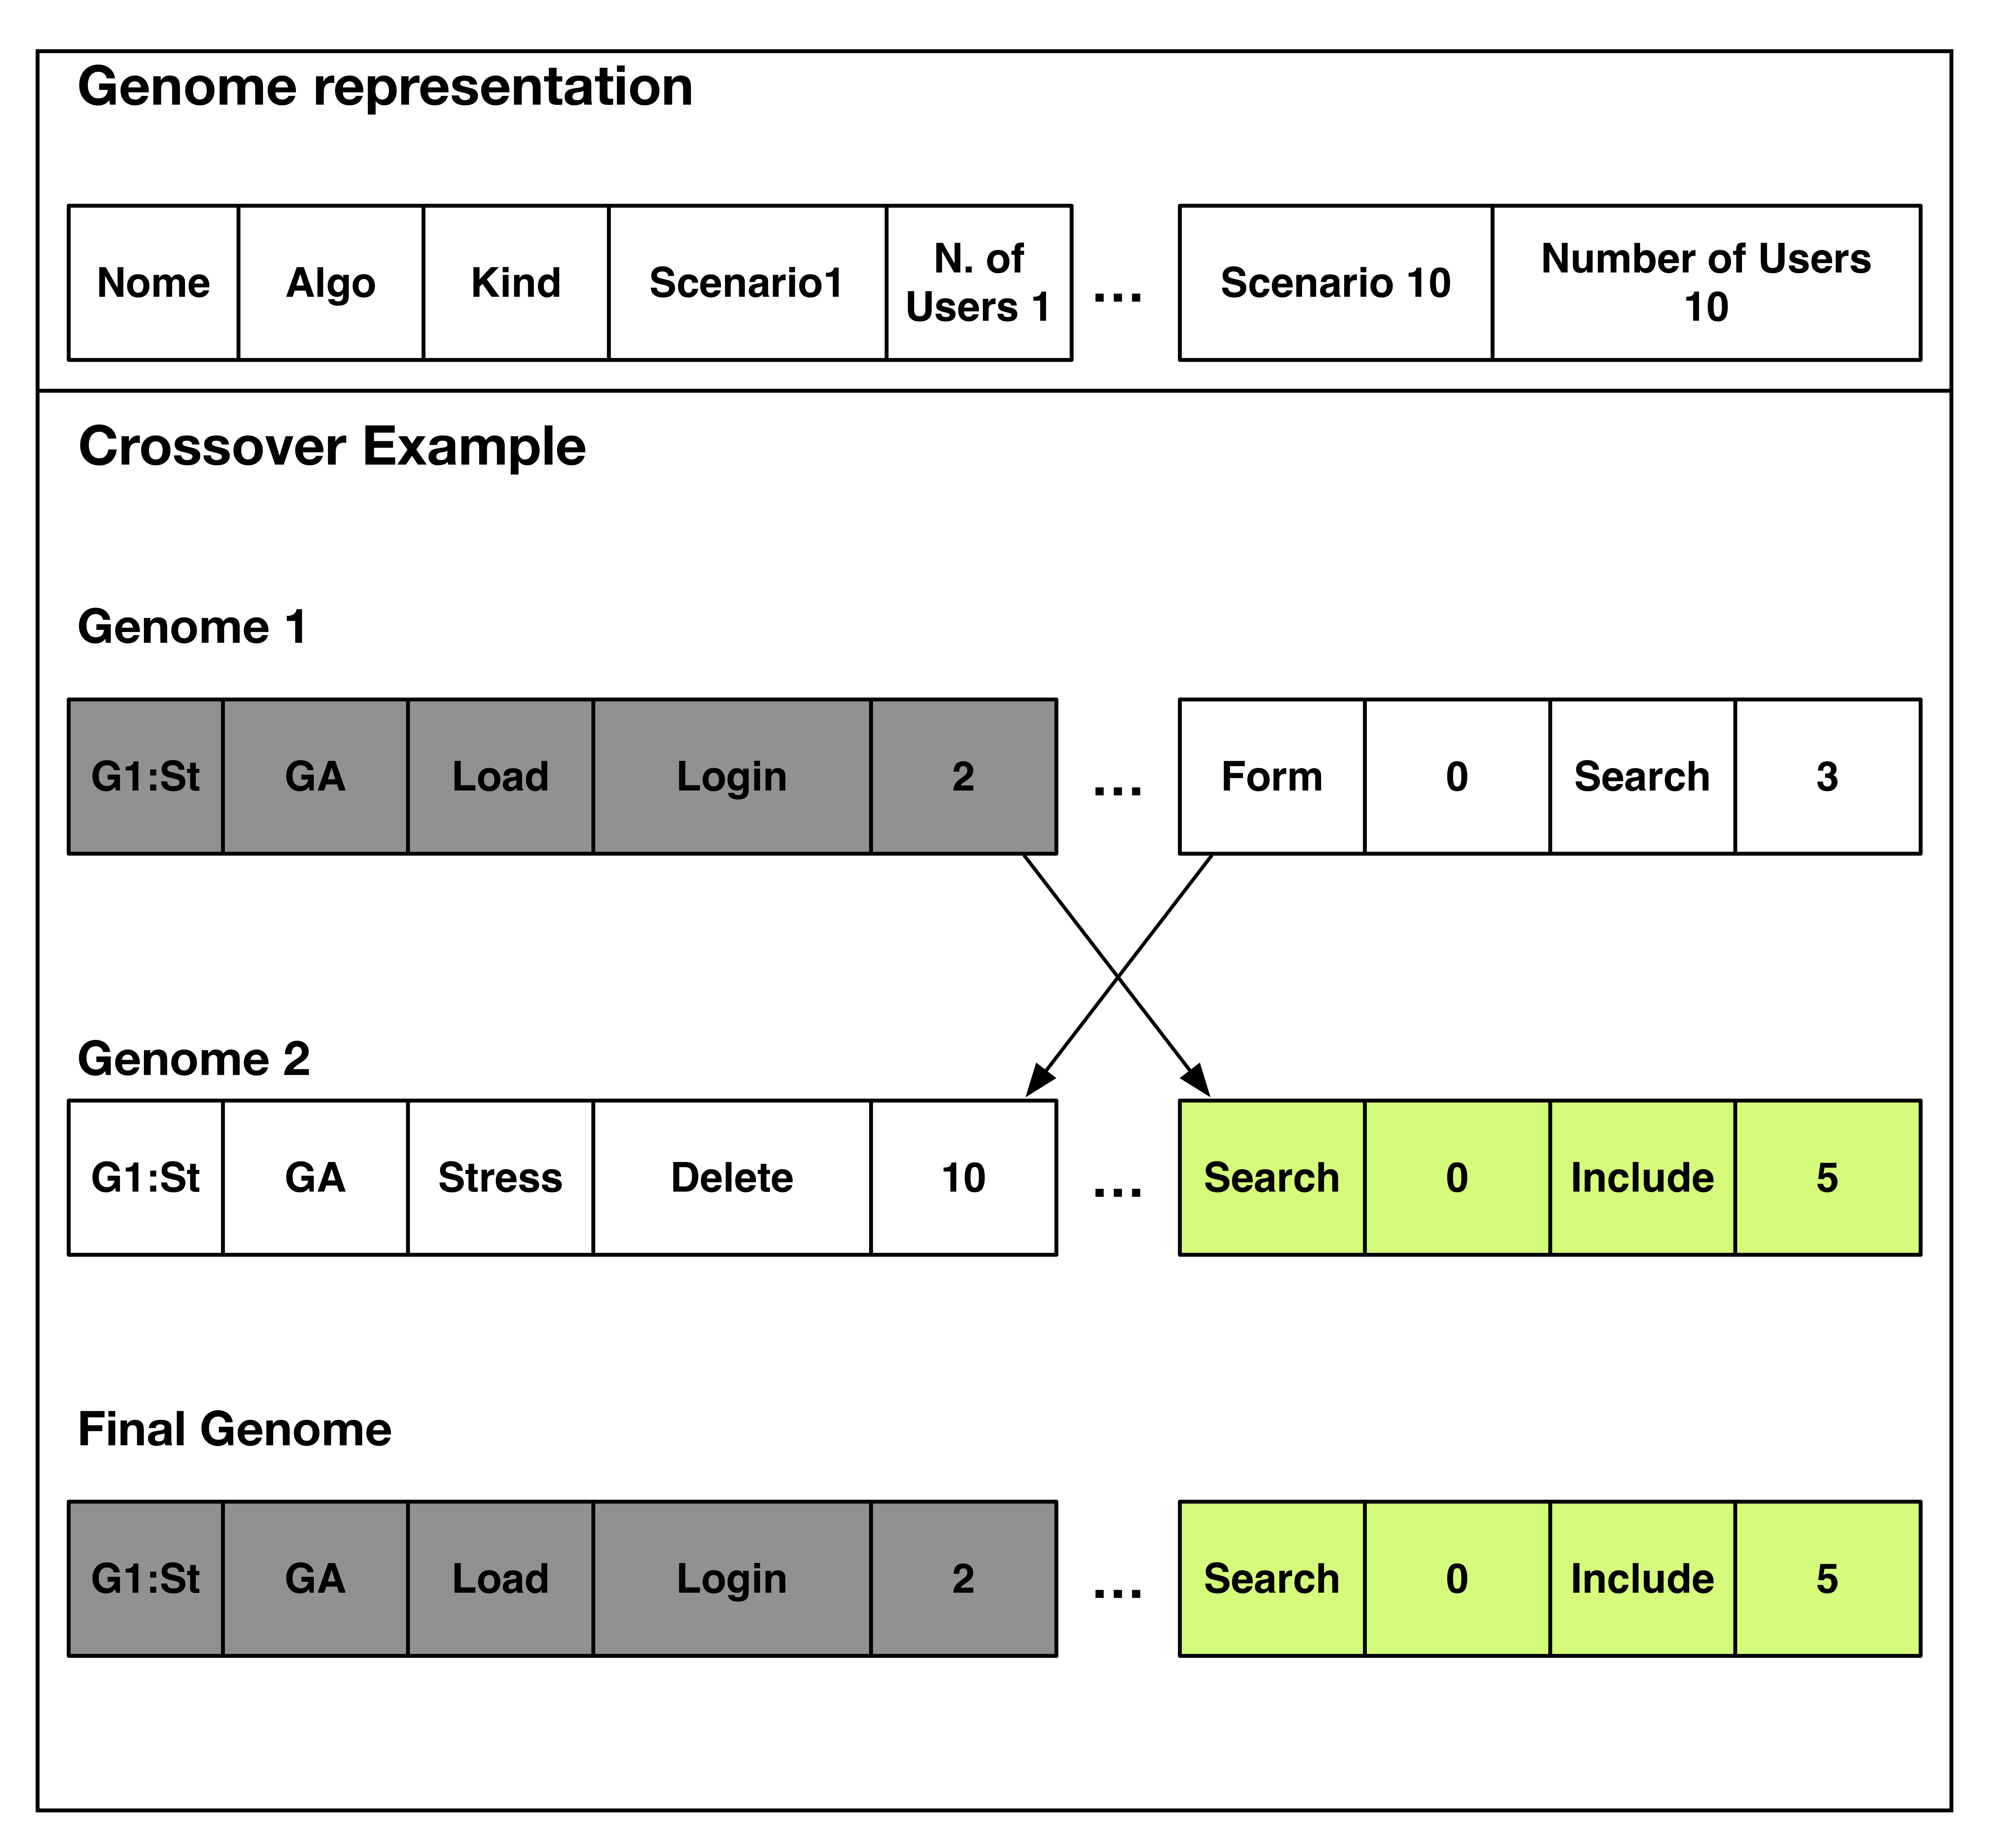
\includegraphics[width=0.5\textwidth]{./images/genomerepresentation.png}
\label{fig:genomarepresentation}
\end{figure}


\subsubsection{Objective (Fitnesse) Function}

The IAdapter is a tool to be used with the independent testing teams in various situations where the team has no direct access to the environment where the application under test was installed. Therefore,  The IAdapter uses a measurement approach to the definition of the fitnesse function. The fitnesse function applied to IAdapter solution is governed by the following equation:

\begin{equation}
\begin{aligned}
fit=90percentileweigth* 90percentiletime\\
+80percentileweigth*80percentiletime\\+
70percentileweigth*70percentiletime+\\
maxResponseWeigth*maxResponseTime+\\
numberOfUsersWeigth*numberOfUsers-penalty
\end{aligned}
\end{equation}

The IAdapter's fitnesse function uses a series of adaptable User-defined weights. These weights make it possible to customize the search plugin funcionality. The penalty is applied when a application under test responds responds in a longer time than the level of service.

\subsubsection{Tabu Search and Simulated Annealing algorithms }

The Fig. \ref{fig:neighbourtaby} shows the strategy used by IAdapter to obtain the neighbours in the Tabu Search and Simulated Annealing algorithms.  The neighbours are obtained by the modification of a single cromossome (scenario or  number of users) in the genotype.

\begin{figure}
\caption{Tabu Search and Simulated Annealing neighbour strategy}
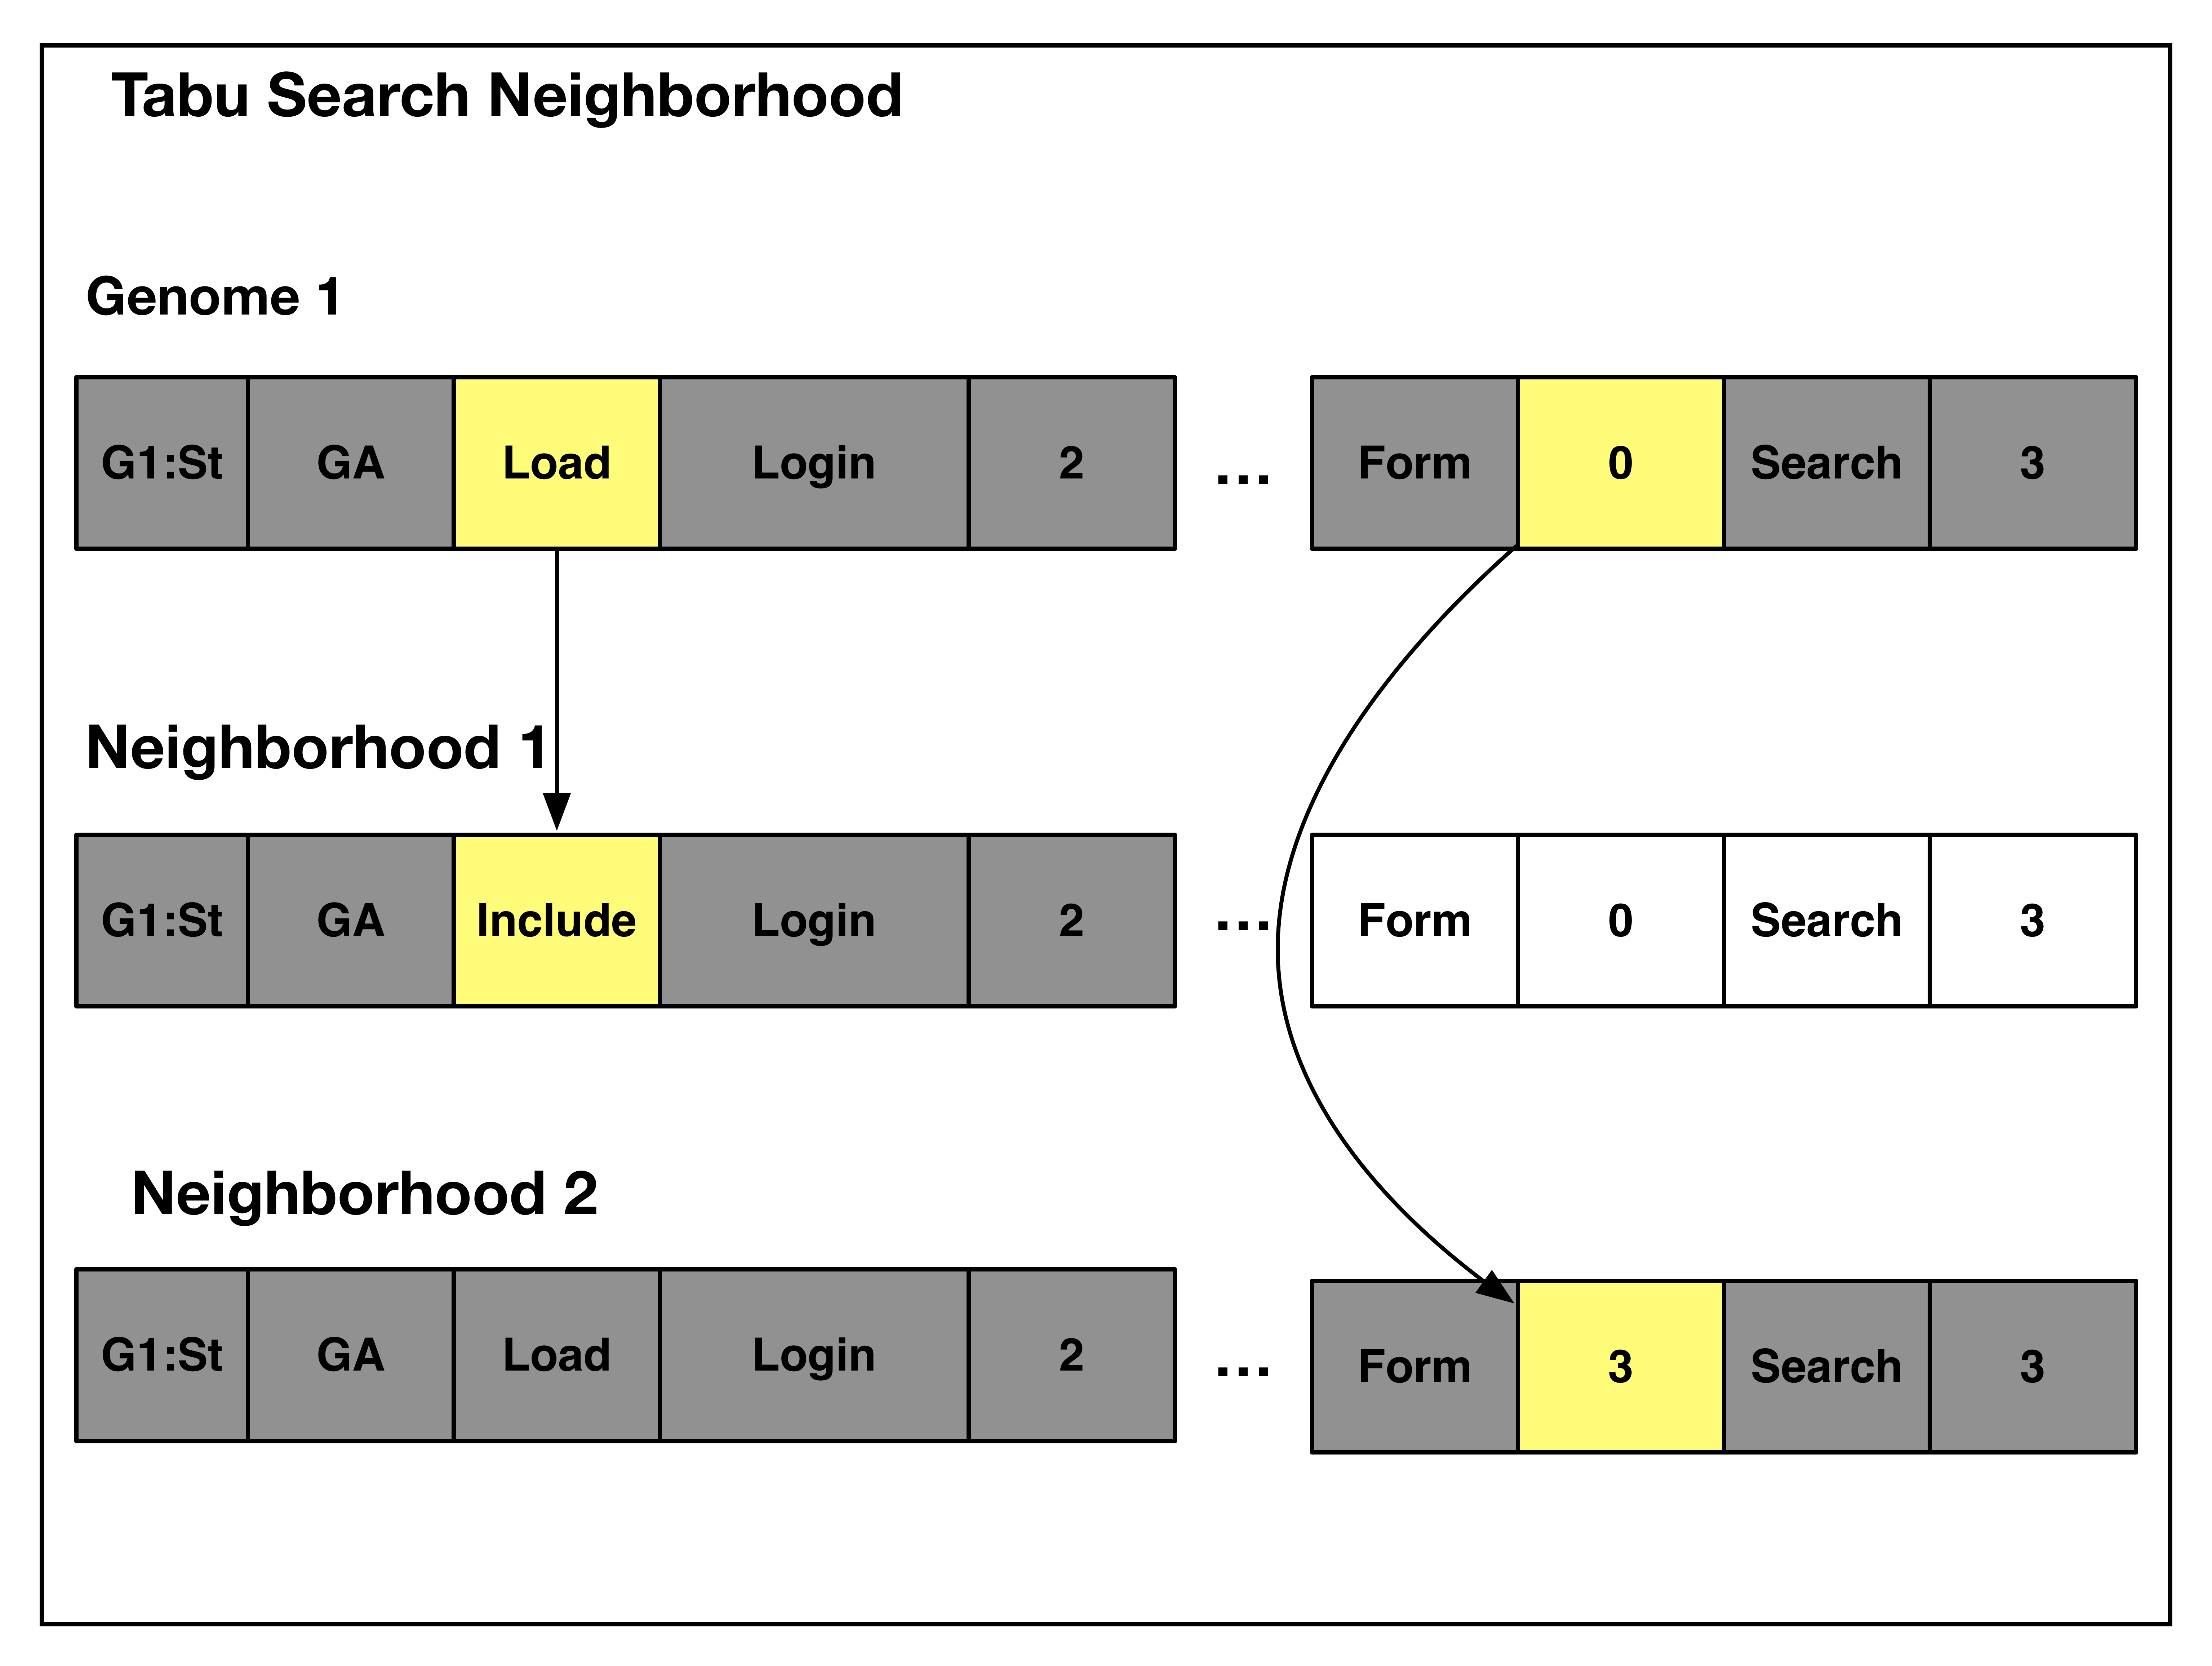
\includegraphics[width=0.5\textwidth]{./images/TabuNE.png}
\label{fig:neighbourtaby}
\end{figure}

The IAdapter uses a tabu list of fixed size and expires every two generations. In the Simulated Annealing algorithm, the temperature variable is represented by the number of users.


\subsection{IAdapter Components}

The JMeter have components organized  in a hierarchical manner. The IAdapter plugin provides three main components:

\begin{itemize}
\item WorkLoadThreadGroup;
\item WorkLoadSaver; and
\item WorkLoadController.
\end{itemize}
 
The WorkLoadThreadGroup is a component that creates an initial population and configure the algorithms used in IAdapter . The Fig. \ref{fig:tela1iadapter} presents the main screen of the WorkLoadThreadGroup component. The component has a name (Fig. \ref{fig:tela1iadapter} -1), a set of configuration tabs (Fig. \ref{fig:tela1iadapter} -2), a list of individuals by generation (Fig. \ref{fig:tela1iadapter} -3), a button to generate an initial population (Fig. \ref{fig:tela1iadapter} -4) and a button to export the results (Fig. \ref{fig:tela1iadapter} -5).

\begin{figure}[h]
\caption{WorkLoadThreadGroup component}
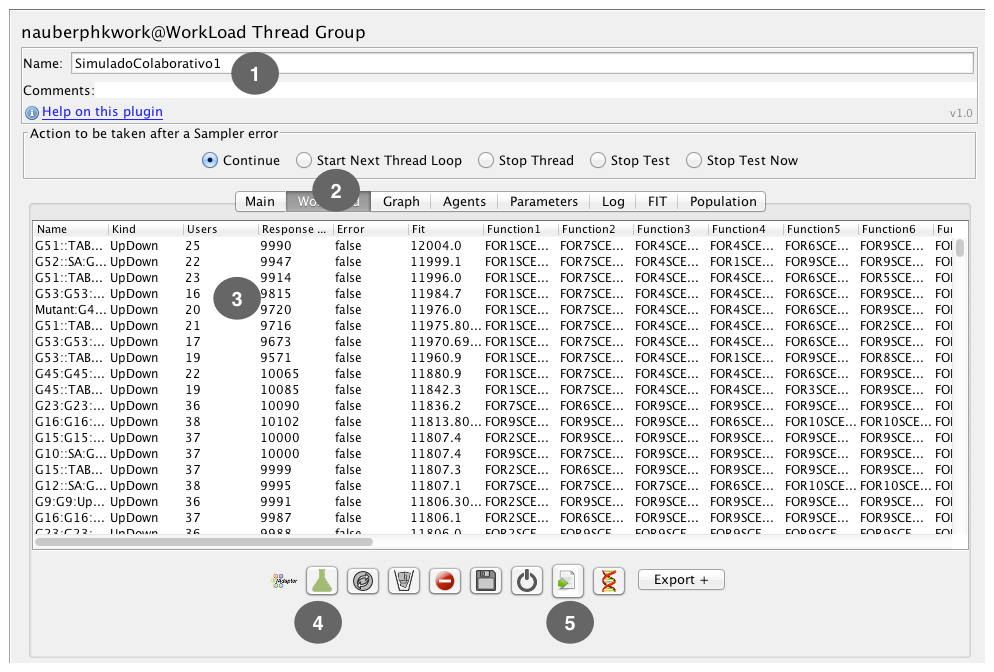
\includegraphics[width=0.5\textwidth]{./images/tela1iadapter.png}
\label{fig:tela1iadapter}
\end{figure}

The WorkLoadSaver component is responsible for saving all data in the database. The operation of the component is simple and only requires its inclusion in the test script. The WorkLoadController represents a scenario of test. The WorkLoadController represents a scenario of test. All actions necessary to test a application should be included in this component. All instance of the component need to login in the application under test and return the application to it's original state.
%\section{Experiments}

This section presents two experiments. The first one has been applied in an emulated component and The second experiment has been applied in an installed Moodle application. The experiments used this fitnesse function:

\begin{equation}
\begin{aligned}
fit=0.9* 90percentiletime\\
+0.1*80percentiletime\\+
0.1*70percentiletime+\\
0.1*maxResponseTime+\\
0.2*numberOfUsers-penalty
\end{aligned}
\end{equation}

The fitnesse function used in the experiments intended to find individuals with the highest percentile of 90\%, followed by individuals with higher percentile time of 80\% and 70\%, maximum response time and number of users.

The experiments have  emulated 27 generations with 300 executions by generation (100 times for each algorithm),  generating 300 news individuals. The experiments had used a initial population of 100 individuals. The Genetic Algorithm used the top 10 individuals from each generation to the crossover operation. The Tabu List has been configured with the size of 10 individuals and expire every 2 generations.  The mutation operation was applied to 10\% of the population on each generation. 

\subsection{First Experiment- Emulated Class Test}

The first experiment aimed to apply performance, load and stress testing in a simulated component. The purpose of using a simulated component is able to perform a greater number of generations in a shorter time available and eliminate variables such as the use of databases and application servers. The first experiment used a test class  named SimulateConcurrentAccess. These class have a static variable named \textit{x} and a set of methods that uses the variable in a synchronized context ( Listing \ref{classsimulated}).

\lstdefinestyle{outline}{
		language=Java,
         basicstyle=\scriptsize\ttfamily,
         numberstyle=\tiny,
         numbersep=5pt,
         tabsize=2,
         extendedchars=true,
         breaklines=true,
         keywordstyle=\color{black}\bf,
         frame=b,  % <<<<<<<<<<<<<<<<<<<<<<<<<<
         stringstyle=\color{green!40!black}\ttfamily,
         showspaces=false,
         showtabs=false,
         numbers=left,
         xleftmargin=17pt,
         framexleftmargin=17pt,
         framextopmargin=1pt, % <<<<<<<<<<<<<<<<<<<<<<
         showstringspaces=false,
         %backgroundcolor=\color[RGB]{200,200,200},
         belowcaptionskip=0pt
}

\begin{lstlisting}[style=outline,caption={SimulateConcurrentAcess class},label=classsimulated]
public class SimulateConcurrentAccess {
  @Test
  public void test() {		
    synchronized (StaticClass.class) {
			for (int i = 0; i <= 1000; i++) {
				StaticClass.x += i;
			}
			StaticClass.x = 0;
		}
	}
\end{lstlisting}


Fig.\ref{fig:exp1bestresults} presents the best results in 27 generations applied in the first experiment . The Figure shows the results obtained with the algorithms with and without collaboration. The $x$ axis  represents the generation number and the $y$ axis represents the best fitnesse value obtained until the current generation. The results of the experiment showed that the use of cooperation between the three algorithms resulted in find individuals with better fitnesse values.

\begin{figure}[h]
\centering
\caption{Best results obtained in 27 generations}
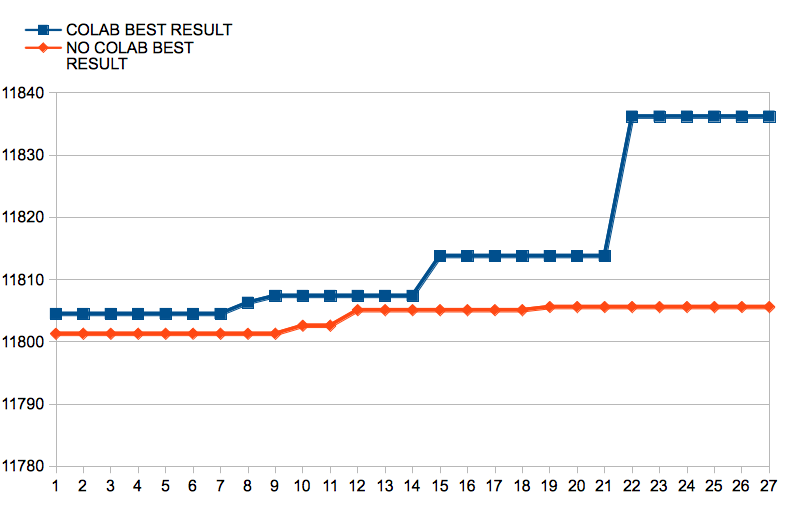
\includegraphics[width=0.5\textwidth]{./images/exp1bestresults.png}
\label{fig:exp1bestresults}
\end{figure}
The table \ref{tab:averagefirst} presents the results obtained by Genetic Algorithm (GA) and TABU Search (TS) from 27 generations in the first experiment. The four columns of the table represent the use of GA a TS with collaboration  (Col) and with no collaboration (No).  The values are the average of the fitnesse value obtained by each algorithm. 

\begin{table}[h]
\centering
\caption{Fitnesse function Average  by algorithm in the first experiment }
\label{tab:averagefirst}
\begin{tabular}{|l|l|l|l|l|}
\hline
G & GA Col  & GA No & TS Col  & TS No\\ \hline
1 & 2855 & 2855 & 2855.00 & 2855\\ \hline
2 & 9545 & 9245 & 10714 & 10591\\ \hline
3 & 9346 & 5535 & 10718 & 8932\\ \hline
4 & 3827 & 5957 & 8527 & 3000\\ \hline
5 & 5880 & 10738 & 8527 & 3000\\ \hline
6 & 11801 & 9583 & 8797 & 8650\\ \hline
7 & 4984 & 9241 & 9985 & 4139\\ \hline
8 & 9063 & 10085 & 9985 & 5256\\ \hline
9 & 8915 & 9099 & 9998 & 6779\\ \hline
10 & 9945 & 10281 & 10163 & 6832\\ \hline
11 & 9991 & 8831 & 10352 & 9048\\ \hline
12 & 10535 & 10578 & 10425 & 9819\\ \hline
13 & 10325 & 10383 & 10319 & 9652\\ \hline
14 & 11414 & 7197 & 9948 & 9394\\ \hline
15 & 10754 & 7189 & 10388 & 1701\\ \hline
16 & 10632 & 7309 & 9878 & 4193\\ \hline
17 & 10108 & 8762 & 10007 & 5300\\ \hline
18 & 4769 & 8360 & 10007 & 5430\\ \hline
19 & 7397 & 9527 & 5508 & 5716\\ \hline
20 & 8418 & 10378 & 4816 & 7417\\ \hline
21 & 9526 & 10301 & 9243 & 8940\\ \hline
22 & 7128 & 9595 & 8095 & 9872\\ \hline
23 & 8519 & 9981 & 9332 & 11024\\ \hline
24 & 10053 & 9647 & 10138 & 9479\\ \hline
25 & 8759 & 11045 & 9313 & 10668\\ \hline
26 & 9601 & 10798 & 8629 & 10837\\ \hline
27 & 6352 & 10739 & 10367 & 9754\\ \hline
\end{tabular}
\end{table}

The signed-rank Wilcoxon non-parametrical procedure was used for comparing the results. The test showed that there was no significant improvement in the use of collaborative approach to the use of genetic algorithms. However , the use of collaborative approach showed significant improvement in the use of the algorithm TS and in turn the final result obtained.

\begin{lstlisting}[style=outline,caption={Result obtained by the  Wilcoxon test with the results of TS Colab and TS No},float,label=classsimulated]

Result Details

W-value: 70
Mean Difference: -1497.04
Sum of pos. ranks: 281
Sum of neg. ranks: 70

Z-value: -2.6795
Mean (W): 175.5
Standard Deviation (W): 39.37

Sample Size (N): 27

Result 1 - Z-value

The Z-value is -2.6795. The p-value is 0.00736. The result is significant at p≤ 0.05.

Result 2 - W-value

The W-value is 70. The critical value of W for N = 26 at p≤ 0.05 is 98. Therefore, the result is significant at p≤ 0.05.
\end{lstlisting}


\subsection{Second Experiment- Moodle Application Test}

The second experiment uses a Moodle application installed in a machine with 500 Gb of hard disk and 8 Gb of memory.The study used six application scenarios:

\begin{itemize}
\item PostDeleteMessage- This scenario post and delete messages in the moodle application.
\item MyHome- This scenario access the user's homepage of the application.
\item Login- This scenario are responsible by the user authentication of the application.
\item Notifications- This scenario enter in the notification page of each user.
\item Start Page- Initial start page of the application.
\item Badge- This scenario enter in the Badge page.
\end{itemize}

The maximum tolerated response time in test was 30 seconds.  Any  individuals that obtained a time longer than the stipulated maximum time suffered penalties.  The whole process of stress and performance tests, which took three days and about 1800 executions, was carried out without the need for monitoring of a test designer. The tool have  selected automatically the next scenarios to be run up to the limit of six generations previously established. 

The Fig. \ref{fig:g13moodle} presents the resume of the results obtained in the six generations of the experiment. The results are grouped by algorithm type (colaboration or non colaboration) and generation.  The columns presents the fitnesse average value by each algorithm. The results of the experiment showed that The TABU search algorithm found most of the best individuals. The use of cooperation between the three algorithms resulted in better fitnesse values in most experiments. The experiment succeeded in finding 29 individuals where the maximum time expected by the application was obtained.  The Fig. \ref{fig:individuals} has four individuals who have obtained the maximum time expected by the application.

\begin{figure}[h]
\centering
\caption{Example of individuals obtained in the second experiment}
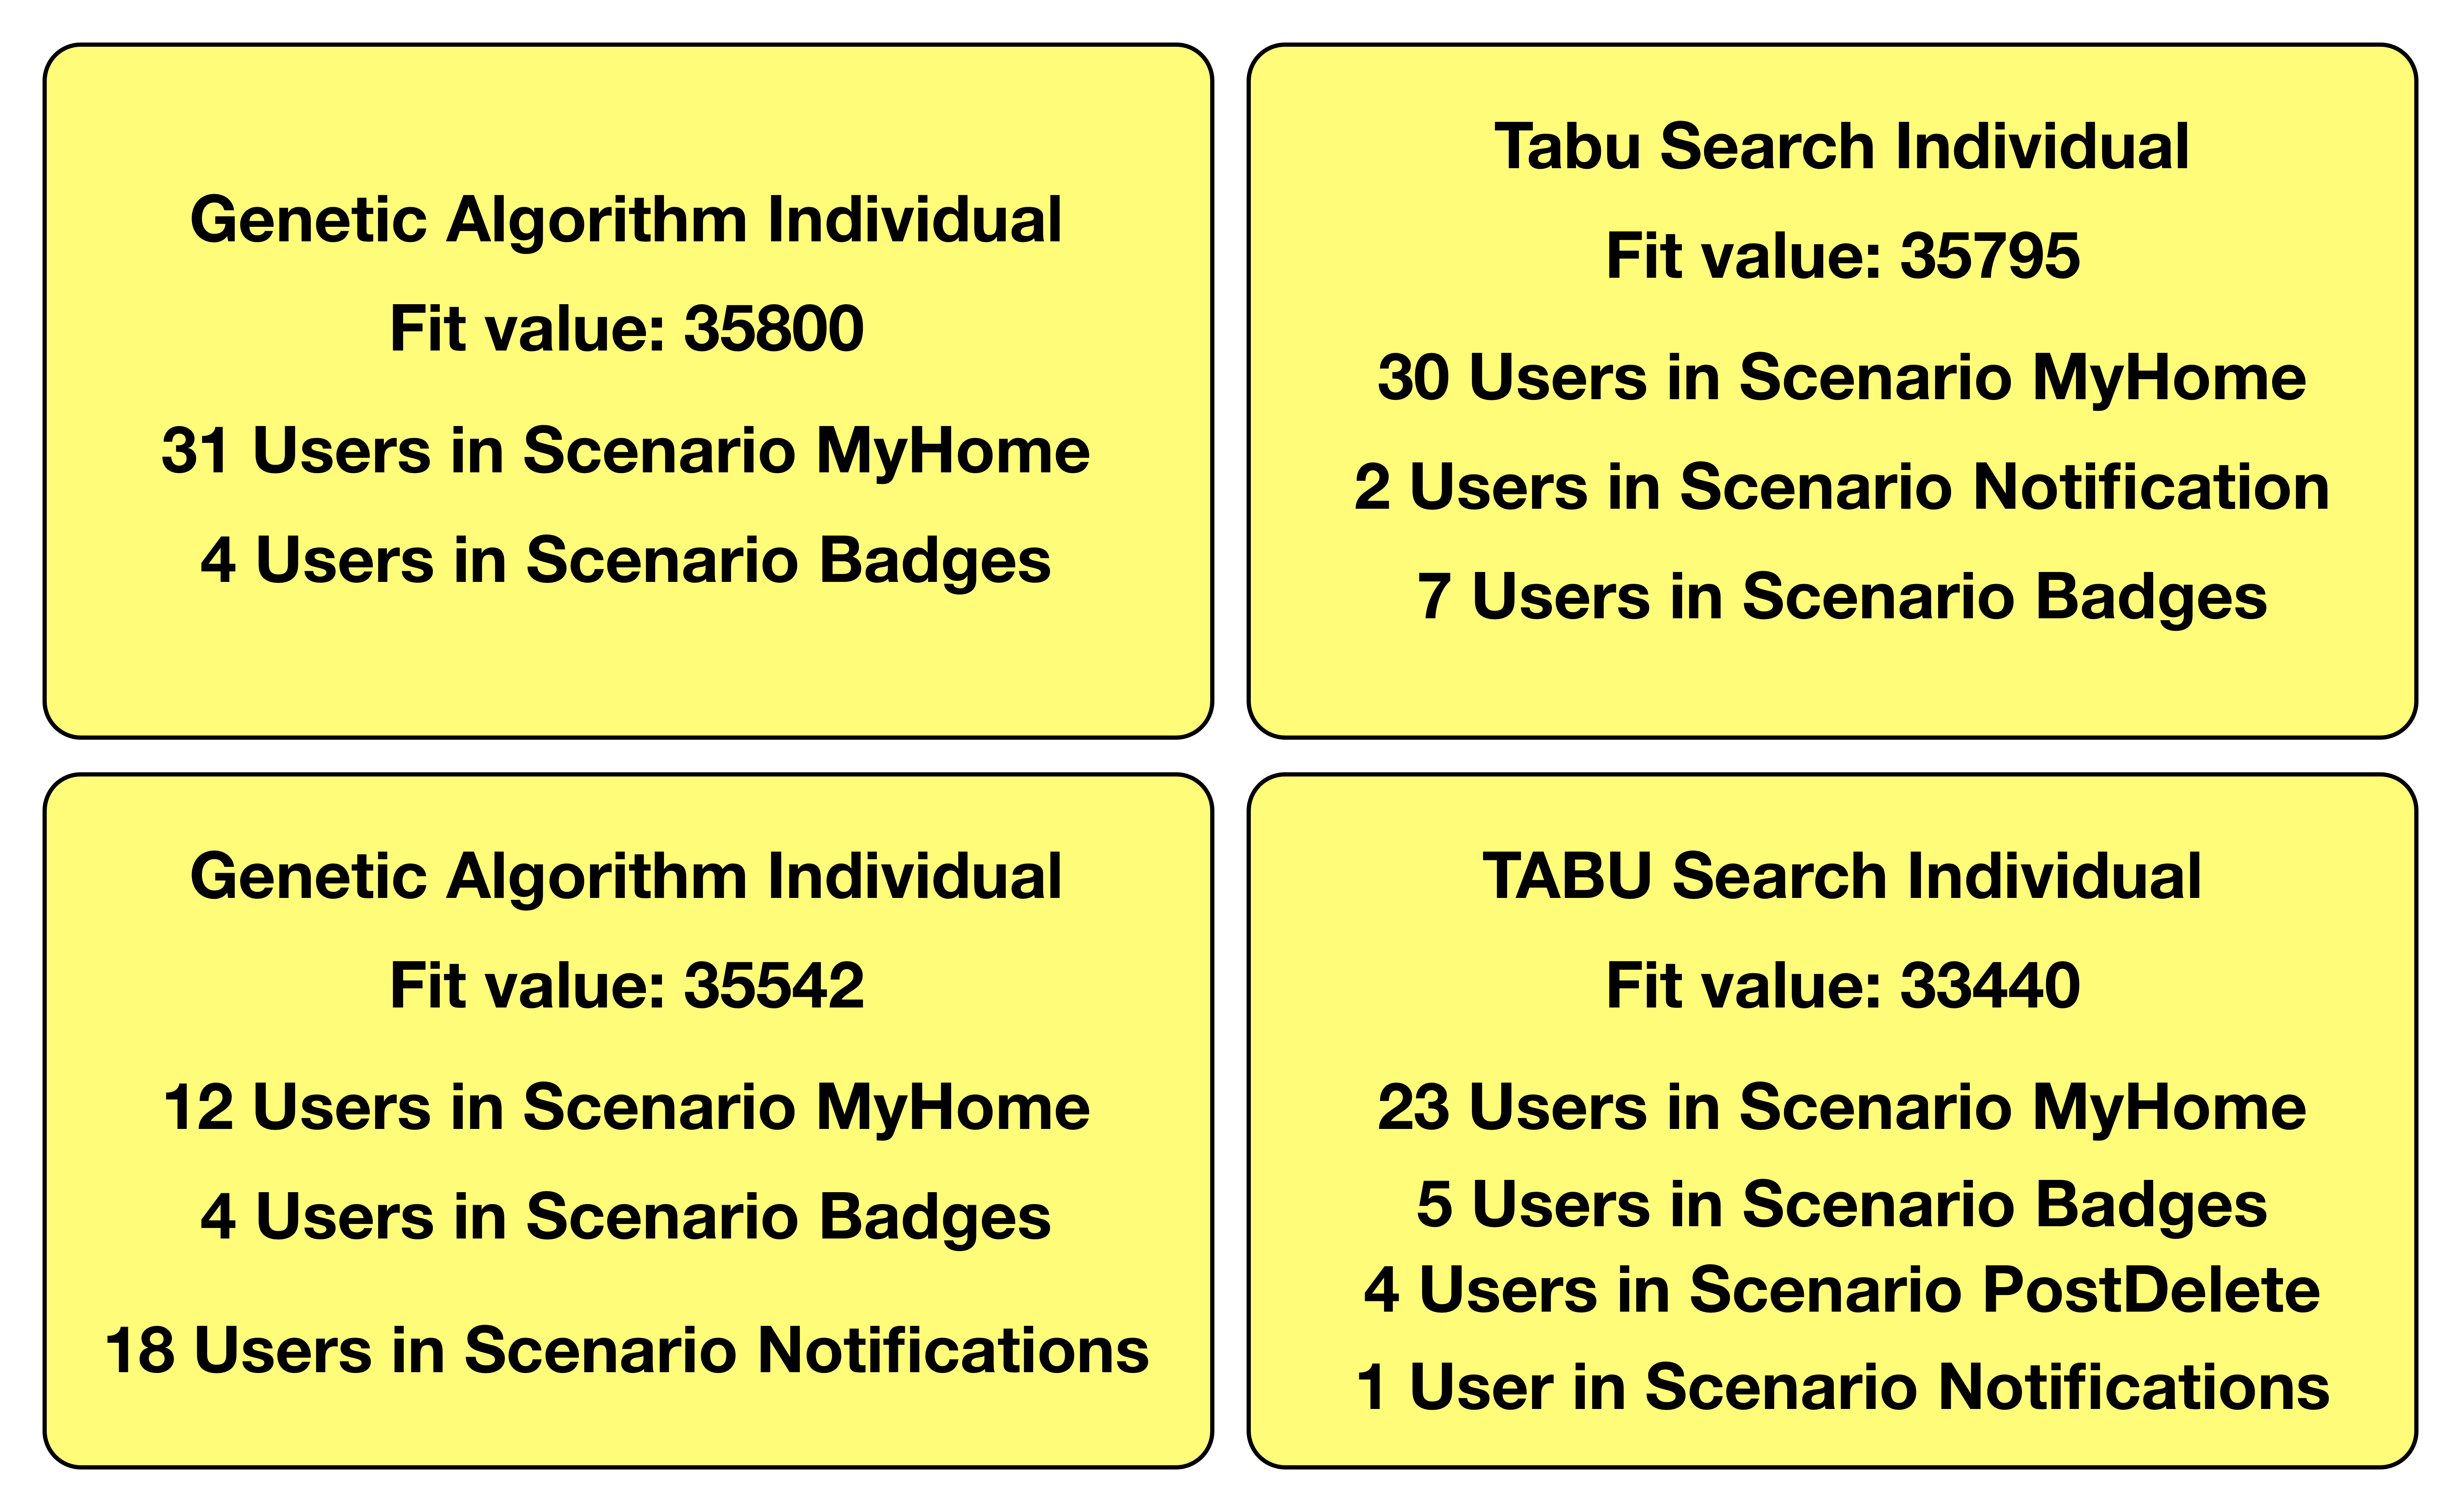
\includegraphics[width=0.5\textwidth]{./images/individuals.png}
\label{fig:individuals}
\end{figure}

\begin{figure*}[h]
\centering
\captionof{figure}{The results for the first generations (1-6) of tests applied in the Moodle application}
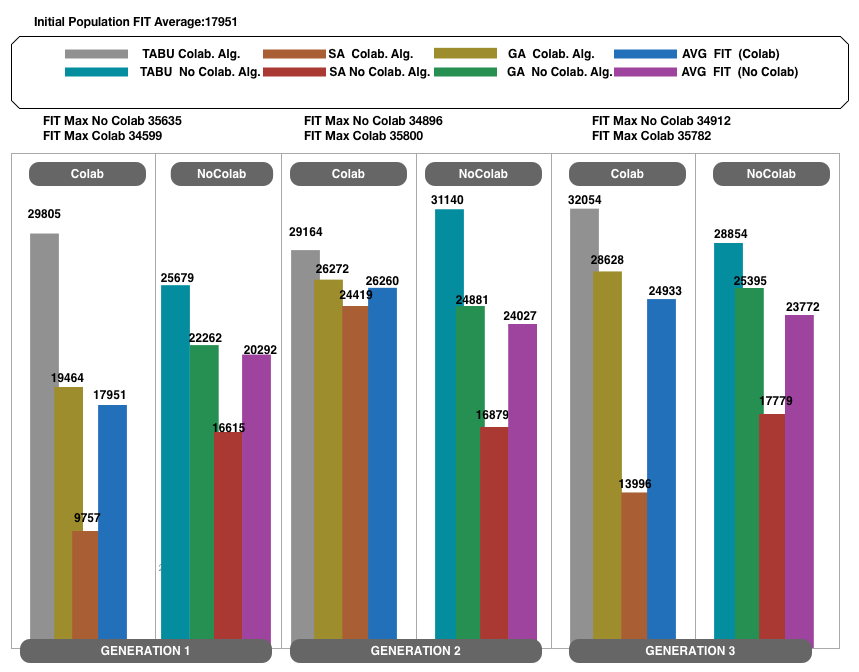
\includegraphics[width=0.8\textwidth]{./images/GENERATIONS1.png}
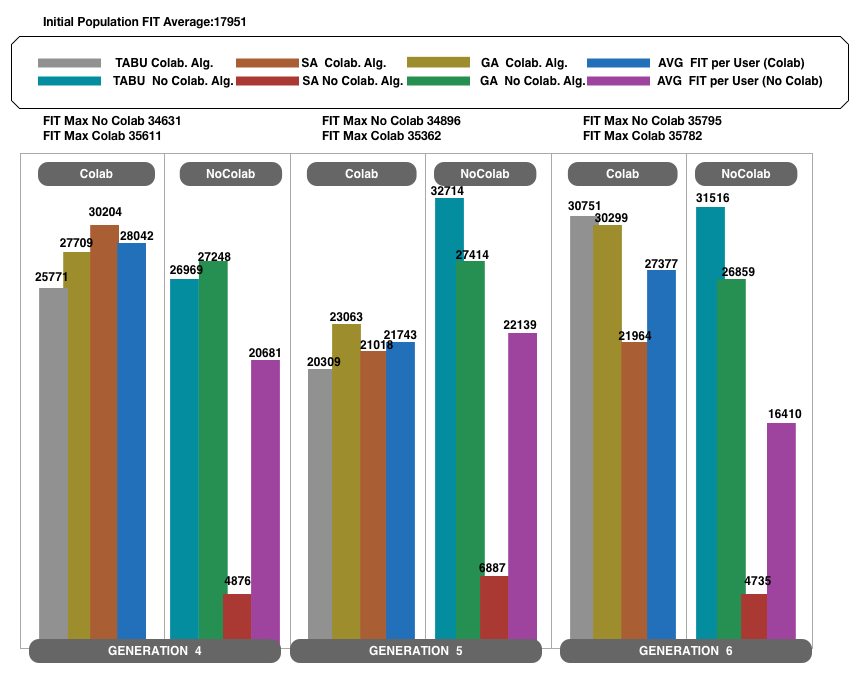
\includegraphics[width=0.8\textwidth]{./images/GENERATIONS2.png}
\label{fig:g13moodle}
\end{figure*}

%\section{Contributions and Comparative Analysis}

The main contributions of the research are:

\begin{itemize}
\item The presentation of an approach that uses a committee of algorithms (GA, SA and TS);
\item The use of Tabu Search Algorithm ( TS ) to find scenarios that break the  service level defined by the application under test;
\end{itemize}

The secondary contributions of the research are:

\begin{itemize}
\item The provision of a JMeter plugin for conducting performance, load or stress  testing.
\item The extension of the survey conducted by  Afzal et al. in the Load, Performance and Stress testing context \cite{Afzal2009}
\item The automation of the  load, performance or stress test execution process.
\end{itemize}

The Figure \ref{fig:comparison} presents the comparison between this research and the others studies found in the systematic review. The IAdapter presents a solution that uses a committee of algorithms in a measurement approach using a functional tool (JMeter with IAdapter plugin).

\begin{figure}[h]
\centering
\includegraphics[width=0.5\textwidth]{./images/comparativo.png}
\caption{
Distribution of the researches over range of applied metaheuristics}
\label{fig:comparison}
\end{figure}
%\section{Conclusion}

This paper presented a approach of use combinatorial optimization algorithm in load, performance and stress testing. The study performed a systematic review ; the development of a plugin and two experiments. The IAdapter is a JMeter Plugin to perform evolutionary load, performance or stress tests. The IAdapter plugin makes it possible to create a generative model that evolves during the test. The first experiment has been applied in an emulated component and the second experiment has been applied in an installed Moodle application.  The collaborative approach has obtained better fit values in both experiments. 

The main contributions of the research are:

\begin{itemize}
\item The presentation of an approach that uses a hybrid metauristc approach;
\item The use of Tabu Search Algorithm ( TS ) to find scenarios that break the  service level defined by the application under test;
\end{itemize}

The secondary contributions of the research are:

\begin{itemize}
\item The provision of a JMeter plugin for conducting performance, load or stress  testing.
\item The automation of the  load, performance or stress test execution process.
\end{itemize}

Among the future work of the research, we can highlight the use of new combinatorial optimization algorithms such as Very large-scale neighborhood search.
%\import{sections/}{texfiles/planning.tex}
%\import{sections/}{texfiles/loadtest.tex}
%\import{sections/}{texfiles/workload.tex}
%\import{sections/}{texfiles/jmeter.tex}
%\import{sections/}{texfiles/evolutionary.tex}
%\import{sections/}{texfiles/iadapter.tex}
%\import{sections/}{texfiles/experiments.tex}
%\import{sections/}{texfiles/comparative.tex}
%\import{sections/}{texfiles/conclusion.tex}

%\section*{Reference}

%% The Appendices part is started with the command \appendix;
%% appendix sections are then done as normal sections
%% \appendix

%% \section{}
%% \label{}

%% References
%%
%% Following citation commands can be used in the body text:
%% Usage of \cite is as follows:
%%   \cite{key}          ==>>  [#]
%%   \cite[chap. 2]{key} ==>>  [#, chap. 2]
%%   \citet{key}         ==>>  Author [#]

%% References with bibTeX database:

\section*{Reference}

\bibliographystyle{model1-num-names}
%\bibliographystyle{plain}
\bibliography{sample}

%% Authors are advised to submit their bibtex database files. They are
%% requested to list a bibtex style file in the manuscript if they do
%% not want to use model1-num-names.bst.

%% References without bibTeX database:

% \begin{thebibliography}{00}

%% \bibitem must have the following form:
%%   \bibitem{key}...
%%

% \bibitem{}

% \end{thebibliography}


\end{document}

%%
%% End of file `elsarticle-template-1-num.tex'.